\documentclass[12pt]{article}
\usepackage[utf8]{inputenc}
\usepackage[letterpaper,margin=1.0in]{geometry}
%% Some formatting stuff
\usepackage{authblk}
\usepackage{fancyhdr}
%\usepackage{lineno}
\usepackage{siunitx}
\usepackage{hyperref}
\usepackage{booktabs}
\usepackage{multirow}
\pagestyle{fancy}
\setlength{\headheight}{14.5pt} % Fix fancyhdr warning
% Custom citep command for biblatex
\newcommand{\citep}{\parencite}
\fancyhead[R]{\textbf{Dosage compensation in squid}}
% for figures
\usepackage{graphicx}
\usepackage{wrapfig}
\usepackage{breakcites}
\usepackage{nameref}
\usepackage{amsmath}
\usepackage{xspace}


%\usepackage[figuresonly,nolists,nomarkers]{endfloat}
%\renewcommand{\processdelayedfloats}{}

\graphicspath{ {./figures/} }

\newcommand{\comment}[1]{{\color{blue} #1}}
\newcommand{\illex}{\textit{Illex illecebrosus}\xspace}

% for hyperlinks
\hypersetup{  
    colorlinks=true,
    citecolor=black,
    urlcolor=cyan,
    linkcolor=blue
    }
\urlstyle{same}

% for highlighting text
\usepackage{xcolor}
\usepackage{soul}

% bibliography
\usepackage[backend=biber,style=authoryear]{biblatex}
\addbibresource{refs.bib}

%\linenumbers
\renewcommand*{\bibfont}{\fontsize{10}{12}\selectfont}


\newcommand{\beginsupplement}{%
    \setcounter{table}{0}
    \renewcommand{\thetable}{S\arabic{table}}%
    \setcounter{figure}{0}
    \renewcommand{\thefigure}{S\arabic{figure}}%
}

\def\changemargin#1#2{\list{}{\rightmargin#2\leftmargin#1}\item[]}
\let\endchangemargin=\endlist 

\title{Z chromosome dosage compensation in the northern shortfin squid, \illex}
\author[1, 2]{Scott T. Small}
\author[1, 2]{Silas Tittes}
\author[3,4]{Thomas Desvignes}
\author[1,4]{John H. Postlethwait}
\author[1, 2]{Andrew D. Kern}
\affil[1]{\small{University of Oregon, Institute of Ecology and Evolution}}
\affil[2]{\small{University of Oregon, Department of Biology}}
\affil[3]{\small{Department of Biology, University of Alabama at Birmingham}}
\affil[4]{\small{University of Oregon, Institute of Neuroscience}}

\date{\small{\today{}}}

\begin{document}

\maketitle

\section*{Introduction}
Dosage compensation is the regulatory mechanism by which gene expression between
individuals with differing numbers of sex chromosomes is equalized. 
In organisms with heteromorphic sex chromosomes, such as XX/XY or ZZ/ZW systems,
gene content asymmetries can disrupt dosage-sensitive processes unless expression
levels are balanced. 
Multiple lineages have independently evolved mechanisms to address this imbalance. 
For example, in mammals, one X chromosome is transcriptionally silenced in females via the XIST long non-coding RNA \citep{lyon1961gene, brockdorff2015dosage}; 
in Drosophila, males upregulate their single X chromosome via the Male-Specific Lethal (MSL) complex \citep{lucchesi2015dosage}; 
and in Caenorhabditis elegans, hermaphrodites downregulate both X chromosomes by half \citep{meyer2005x}. 
These strategies ensure dosage parity with the heterogametic sex and preserve essential gene balance during development.

Despite its evolutionary utility, dosage compensation is not ubiquitous or mechanistically uniform. 
In birds (ZZ/ZW), females often exhibit lower expression of Z-linked genes 
compared to males, indicating incomplete compensation \citep{mank2009w, itoh2007dosage}.
Similar patterns are seen in Lepidoptera and some reptiles, 
where partial or gene-specific compensation suggests that selection for dosage balance 
is variable across lineages \citep{julien2012mechanisms, gu2017evolution}. 
The degree of compensation often correlates with the age and extent of degeneration
of the sex-limited chromosome. 
These observations imply that dosage compensation may evolve progressively 
and that partial regulation may suffice in lineages with relatively homomorphic or 
recently evolved sex chromosomes.

Cephalopods, long thought to lack genetic sex chromosomes, have recently emerged as a 
compelling group for studying the evolution of sex chromosomes. 
Classical karyotype analyses failed to reveal heteromorphic sex chromosomes in octopuses, squids, or cuttlefish (CITE), 
leading to hypotheses of environmental or polygenic sex determination. 
However, recent genomic work has overturned this view. 
\citep{coffing2025cephalopod} demonstrated that in octopuses, including \textit{Octopus bimaculoides}, females are hemizygous for a large chromosome (chr17), 
establishing a ZZ/ZO system shared across multiple coleoid lineages. 
This Z chromosome appears to be conserved across squids, cuttlefish, and octopuses, originating over 480 million years ago in a common ancestor. 
Complementary findings by \citep{torrado2025nautilus} in \textit{Nautilus pompilius}—which 
possesses an XX/XY system—highlight the evolutionary diversity of sex determination 
across cephalopods. 
These discoveries position coleoid cephalopods as one of the few known invertebrate 
groups with deeply conserved sex chromosomes.

The presence of a ZO/ZZ system in coleoids raises the question of how these animals
achieve dosage compensation between sexes, 
particularly in females that carry only one Z chromosome. 
Until recently, no studies had examined this issue in any cephalopod. 
\citep{papanicolaou2024z} recently addressed this gap 
by analyzing transcriptomes from \textit{Octopus vulgaris} and \textit{O. sinensis}, and found that Z-linked gene expression was partially compensated in females,
with male-to-female expression ratios averaging ~1.5:1. 
Moreover, they identified a male-specific long non-coding RNA (\textit{Zmast}) 
expressed from the Z chromosome, 
suggesting a potential regulatory mechanism for dosage modulation. 
Notably, Papanicolaou et al. identified not one but two Z-linked long non-coding RNAs
with strikingly sex-specific expression patterns:
\textit{Zmast} (Z-male-specific transcript), which shows 256-fold higher expression in males,
and \textit{Zfest} (Z-female-specific transcript),
an antisense lncRNA at the \textit{Amnionless} locus with 18-fold female-biased expression.
Both lncRNAs are evolutionarily conserved between \textit{O. vulgaris} and \textit{O. sinensis},
species that diverged approximately 2.5 million years ago.
The authors speculate that these lncRNAs may play regulatory roles
analogous to \textit{Xist} in mammals or \textit{roX} genes in \textit{Drosophila},
though their molecular functions remain uncharacterized.
The presence of paired male- and female-specific lncRNAs raises the possibility
of a dual regulatory system governing Z chromosome expression in cephalopods.
The degree of compensation observed in octopus (M:F ratios of approximately 1.04–1.15 across somatic tissues)
is notably more complete than that reported in birds,
where Z-linked genes typically show M:F ratios of 1.4–1.6 \citep{mank2009w}.

While these results reveal the first evidence of dosage compensation in cephalopods,
no comparable studies have been conducted in squids,
leaving open fundamental questions about the prevalence, extent,
and molecular underpinnings of compensation across the group.
Notably, ommastrephid squids such as \illex lack prior genomic or transcriptomic characterization of their sex chromosomes.

In this study, we present a chromosome-scale genome assembly of the northern shortfin squid, 
\illex, and identify its Z chromosome via comparative genomic coverage and synteny analyses. 
We integrate sex-stratified transcriptomic data to assess expression differences between males and 
females for Z-linked genes, and test for evidence of dosage compensation. Finally, we ask if DNA 
methylation contributes to sex-specific regulation on the Z chromosome. T
his work represents the first comprehensive analysis of sex chromosome dosage compensation in any squid 
species and provides critical insight into how ancient sex chromosome systems are regulated in a major 
marine invertebrate lineage.

\section*{Results}
\subsection*{A chromosome-scale genome assembly for \textit{Illex illecebrosus}}
We generated a high-quality chromosome-scale genome assembly for a female \illex individual
using a combination of PacBio HiFi long reads, Illumina short reads, and Hi-C chromatin conformation capture data (Fig. \ref{fig:phylo}A).
The final assembly spanned 4.14 Gb with a contig N50 of 34.71 Mb and scaffold N50 of 75.92 Mb (Table S1).
BUSCO analysis indicated 95.6\% completeness against the metazoan gene set,
demonstrating high assembly quality.
Hi-C scaffolding resolved 46 chromosomes, consistent with the known karyotype of \illex (CITE). 

To create a comprehensive gene annotation, we generated RNA-seq data from multiple tissues
using both Illumina short-read and PacBio Iso-Seq long-read technologies.
Annotation using RNA-seq data from multiple tissues identified 23,192 protein-coding genes,
with a mean intron length of 38 kb.
BUSCO analysis of the protein set indicated 93.1\% completeness (83.2\% single-copy, 6.7\% duplicated),
confirming the high quality of the gene annotation.

Repeat annotation revealed that 58.2\% of the \illex genome consists of repetitive elements (Table S2).
The repeat landscape is dominated by unclassified repeats (28.3\% of the genome),
followed by LINE elements (12.6\%), DNA transposons (6.3\%), and low-complexity regions (5.1\%).
Penelope elements, a clade of retrotransposons common in invertebrates, comprised 3.3\% of the genome.
LTR retrotransposons (2.5\%), SINE elements (1.7\%), and rolling-circle transposons (0.6\%)
were also identified.
In total, we annotated 1,889 distinct classifications of unclassified repeats and
over 7.8 million individual repeat instances across all categories,
reflecting the complex repetitive architecture typical of cephalopod genomes.

\subsection*{Identification of the Z chromosome in \illex}

To identify the Z chromosome in \illex, we performed comparative genomic analyses with other cephalopod species for which sex chromosomes have been characterized.
Whole-genome synteny analysis revealed extensive chromosomal conservation across coleoid cephalopods (Figure 1C).
We compared the \illex assembly to published genomes of \textit{Octopus bimaculoides}, \textit{O. sinensis}, \textit{Euprymna scolopes}, \textit{Sepia esculenta}, \textit{Doryteuthis pealeii}, and \textit{Sepioteuthis oualaniensis}.
Chromosome-scale alignments showed that \illex chromosome 42 exhibits strong synteny with the previously identified Z chromosomes in octopus species and corresponds to conserved linkage groups across squids and cuttlefish.
Despite considerable chromosomal rearrangements, fusions, and fissions across the coleoid phylogeny,
the Z chromosome has maintained its integrity as a distinct chromosomal unit for over 480 million years.
These syntenic relationships, combined with coverage analysis (Figure 1A) showing reduced female-to-male mapping ratios on chromosome 42,
confirm that this chromosome represents the Z chromosome in \illex, consistent with the ZZ/ZO sex determination system described in other coleoid cephalopods.

\begin{figure}[h]
    \centering
    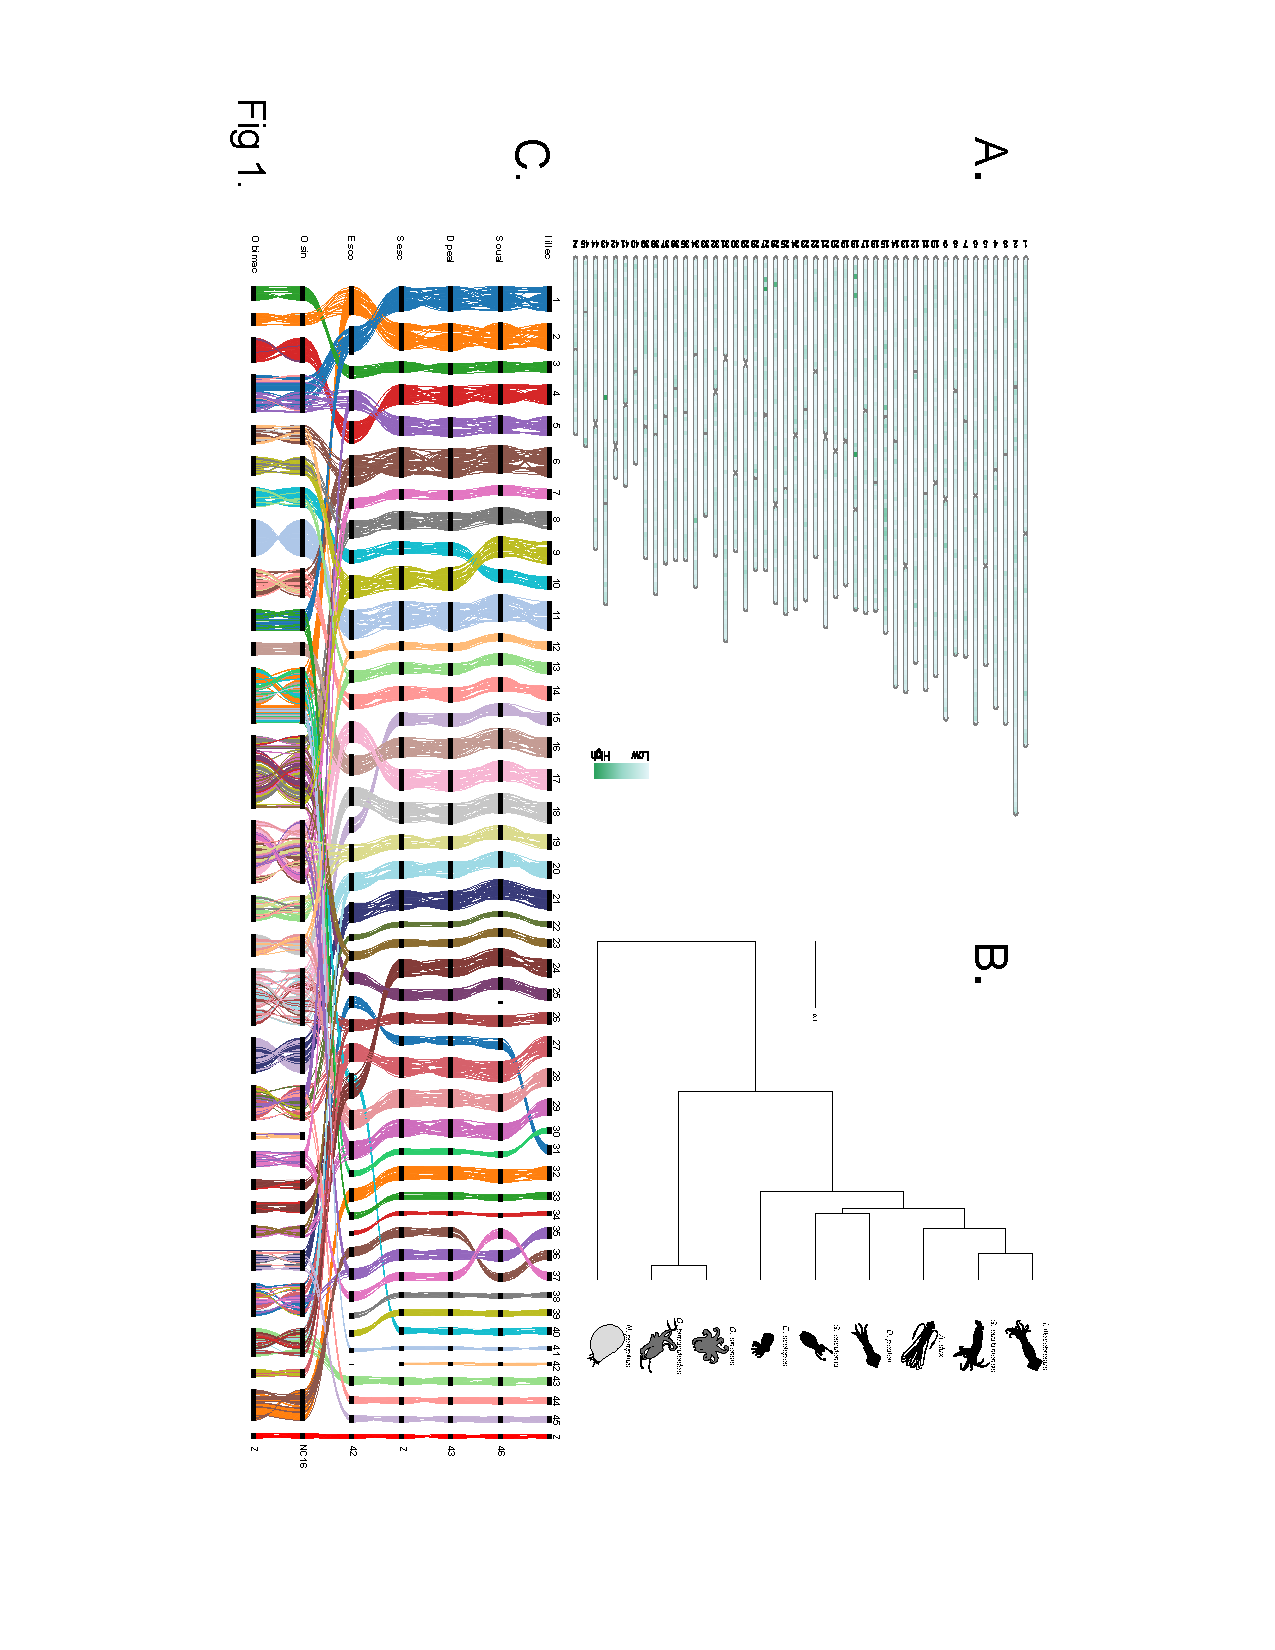
\includegraphics[width=0.8\linewidth, angle=90, origin=c]{figures/fig1.pdf}
    \caption{A chromosomal-scale genome assembly of \textit{Illex illecebrosus} and identification of the Z chromosome
    Panel A: ideogram of the \illex genome assembly showing each chromosome along with the Z chromosome. 
    Shading indicates gene density in 1 Mb windows (darker = higher density).
    Panel B: uncalibrated ultrametic phylogeny of cephalopods used in this study, with phylopic silhouettes for each tip.
    Panel C: Riverine plot showing syntenic relationships between \illex and six other cephalopod species.
    Colors represent chromosomes in each species, with ribbons indicating syntenic blocks.}
    \label{fig:phylo}
\end{figure}

\subsection*{Partial dosage compensation of the Z chromosome}

To assess whether \illex exhibits dosage compensation for Z-linked genes, we analyzed sex-stratified RNA-seq data from multiple tissues.
We quantified gene expression levels across all chromosomes in both males (ZZ) and females (ZO) (Figure 2).
Expression levels on autosomes were comparable between sexes, with median log2(TPM+1) values centered around 2.0-2.5 across all autosomal chromosomes.
In contrast, the Z chromosome showed a distinct pattern: females exhibited systematically lower expression compared to males,
but the female-to-male ratio was substantially greater than the expected 0.5 ratio for complete absence of compensation (Figure 2A,B).

To quantify the degree of compensation, we calculated male-to-female expression ratios (M:F) for Z-linked genes.
The median M:F ratio was approximately 1.5:1, indicating partial dosage compensation where female expression reaches ~67\% of male levels rather than the expected 50\% without any compensation.
Analysis of log2 fold-change distributions confirmed that most Z-linked genes show modest male-biased expression,
with the bulk of genes clustering around a 0.5 log2 fold-change (Figure 2C).
These results demonstrate that \illex exhibits incomplete dosage compensation of the Z chromosome,
similar to patterns observed in octopus species but contrasting with the more complete compensation mechanisms in \textit{Drosophila} and mammals.

\subsection*{DNA methylation patterns on the Z chromosome}

Given the role of epigenetic modifications in gene regulation and dosage compensation in other systems,
we investigated DNA methylation patterns across the \illex genome.
We leveraged PacBio HiFi kinetic signatures from male and female individuals to assess CpG methylation levels.
Genome-wide, we observed a positive correlation between gene expression and methylation levels in both sexes,
with more highly expressed genes showing elevated methylation (Figure 4A; females: r=0.396, p=2.16e-09; males: r=0.318, p=5.10e-06).
This pattern is consistent with gene-body methylation associated with active transcription,
as has been observed in other invertebrates including cephalopods.

When examining sex differences in the relationship between expression and methylation,
we found no significant correlation between male-female expression differences and corresponding methylation differences across Z-linked genes (Figure 4B; r=-0.010, p=0.046).
Methylation levels did not differ substantially between expression quartiles (Figure 4B, right panel),
suggesting that differential DNA methylation is not the primary mechanism driving dosage compensation or sex-biased expression patterns on the Z chromosome.
These findings indicate that while DNA methylation correlates with transcriptional activity genome-wide,
it does not appear to play a major regulatory role in modulating Z chromosome dosage between sexes in \illex.

\subsection*{Sex-biased gene expression on the Z chromosome}

To identify genes with significant sex-biased expression on the Z chromosome,
we performed differential expression analysis of Z-linked genes between males and females.
We identified 23 genes with significant sex-biased expression (Figure 5, Table 1):
10 female-biased genes and 13 male-biased genes.
The majority of sex-biased genes showed modest fold-changes (2-8 fold),
but several genes exhibited extreme sex bias, including XLOC\_014991U (1,364-fold female-biased) and LOC\_00003730 (1,460-fold male-biased).

Functional annotation of sex-biased genes revealed enrichment for several categories relevant to dosage-sensitive processes.
Female-biased genes included two Z-linked long non-coding RNAs (lncRNAs),
including the highly expressed XLOC\_014991U and lncrna-gene-8,
as well as genes involved in neuronal metabolism (SLC5A1), cytoskeletal regulation (FHDC1, Shroom2),
and RNA processing (THOC6, MORN3).
Male-biased genes were enriched for functions in neurotransmission (GABARAP, SLC6A9),
protein turnover (HECTD1, HERC2), cytoskeletal organization (MTUS2, CEP170B),
and RNA splicing (Pasilla).
The presence of highly female-biased lncRNAs on the Z chromosome is particularly intriguing,
as similar Z-linked lncRNAs (e.g., \textit{Zmast} in octopus) have been proposed as candidate regulators of dosage compensation in cephalopods.
The functional enrichment of sex-biased genes for dosage-sensitive processes such as metabolism,
cytoskeletal dynamics, and neurotransmission suggests that incomplete compensation may have phenotypic consequences
or that individual genes have evolved sex-specific regulatory mechanisms.

\subsection*{Identification of a male-biased lncRNA on the Z chromosome}
Among the Z-linked transcripts identified in our RNA-seq analysis,
we noted a long non-coding RNA exhibiting extreme male-biased expression
far exceeding the 2-fold difference expected from gene dosage alone (log2FC = X.XX, p = X.XX).
This dramatic sex bias suggested active regulatory mechanisms
beyond simple copy number effects,
prompting further investigation.
Comparative sequence analysis across squid species revealed a ~400 bp region of striking conservation within the lncRNA.
Secondary structure prediction and covariance analysis demonstrated that this conserved region 
forms a complex stem-loop architecture with strong covariation support, 
indicating evolutionary constraint on RNA structure rather than merely primary sequence (Figure Xa). 
Such conserved structured domains are hallmarks of functional lncRNAs, 
including those involved in dosage compensation such as Xist in mammals and roX in Drosophila.

\paragraph*{The conserved lncRNA domain contains ELAV/SXL family binding sites}
To identify potential regulatory proteins interacting with this lncRNA,
we analyzed the conserved structured region using RBPmap with \textit{Drosophila melanogaster} motifs
(the closest available reference to cephalopods).
This analysis revealed a striking enrichment of binding sites
for the ELAV/SXL family of RNA-binding proteins (Table X).
The most significant predictions included binding motifs for:

\begin{itemize}
\item \textbf{ELAV} (Embryonic Lethal Abnormal Vision):
35 predicted binding sites, with Z-scores up to 3.87 (p $<$ 10$^{-5}$),
concentrated in two U-rich regions (positions $\sim$115-160 and $\sim$420-437)
\item \textbf{SXL} (Sex-lethal):
$\sim$50 predicted binding sites, Z-scores up to 3.98 (p $<$ 10$^{-5}$),
overlapping extensively with ELAV sites
\item \textbf{U2AF50}:
$\sim$60 predicted binding sites, Z-scores up to 3.90 (p $<$ 10$^{-5}$)
\item \textbf{ARET/Bruno}:
15 predicted binding sites in a distinct GU-repeat region (positions $\sim$306-325)
\end{itemize}

The clustering of ELAV and SXL binding predictions is consistent with the known sequence preferences
of these related RBPs,
which share RNA Recognition Motif (RRM) domains that recognize U-rich sequences.
In \textit{Drosophila}, SXL is the master regulator of sex determination and dosage compensation,
while ELAV family proteins regulate mRNA stability in neurons.
The concentration of these binding sites within the conserved structured domain
suggested that protein-RNA interactions may be central to this lncRNA's function.

\paragraph*{ELAV/SXL binding sites are conserved in octopus \textit{Zmast}}
To determine whether the enrichment of ELAV/SXL binding sites is a conserved feature of this lncRNA,
we performed RBPmap analysis on the orthologous \textit{Zmast} sequence from \textit{Octopus vulgaris}.
Strikingly, the octopus \textit{Zmast} showed a nearly identical pattern of RBP binding site enrichment.
We identified $\sim$47 SXL binding sites (Z-scores up to 3.10),
$\sim$30 ELAV binding sites (Z-scores up to 3.29),
and $\sim$37 U2AF50 binding sites (Z-scores up to 3.09),
comparable to the $\sim$60 SXL, $\sim$33 ELAV, and $\sim$61 U2AF50 sites predicted in \illex.
Additional ELAV-family proteins showed consistent enrichment in both species,
including FNE ($\sim$20 sites in octopus, Z-score up to 3.42) and RBP9 ($\sim$23 sites, Z-score up to 3.42).

Notably, comparison of binding site positions between species revealed
that the spatial organization of predicted binding sites is conserved (Table~\ref{tab:rbp_clusters}).
Both sequences exhibit a three-cluster architecture,
with a major U-rich binding site hotspot in the 5$'$ region,
a secondary cluster in the central region,
and a third cluster near the 3$'$ terminus.
When positions are normalized to account for sequence length differences
(~440 nt in \illex versus 411 nt in \textit{O. vulgaris}),
the clusters occur at similar relative locations:
25--36\% of sequence length for cluster 1,
73--78\% for cluster 2,
and 85--100\% for cluster 3.
This positional conservation suggests that the spatial arrangement of SXL/ELAV binding sites
is functionally important,
potentially reflecting structural constraints on protein-RNA complex formation.

\begin{table}[h]
\centering
\caption{Conserved clusters of ELAV/SXL family binding sites in \illex and \textit{O. vulgaris} \textit{Zmast}}
\label{tab:rbp_clusters}
\begin{tabular}{llll}
\toprule
\textbf{Region} & \textbf{\textit{Illex} Position} & \textbf{\textit{O. vulgaris} Position} & \textbf{Notes} \\
\midrule
Cluster 1 & 115--160 & 101--129 & Major U-rich region, highest Z-scores \\
Cluster 2 & 345--361 & 301--320 & Secondary cluster \\
Cluster 3 & 378--437 & 364--400 & 3$'$ terminal region \\
\bottomrule
\end{tabular}
\end{table}

The conservation of both the lncRNA sequence and its predicted protein binding site architecture
between squid and octopus---lineages that diverged over 270 million years ago---strongly
suggests that the regulatory interaction between SXL-family proteins and this lncRNA
is an ancient and functionally constrained feature of coleoid cephalopod dosage compensation.

\paragraph*{Identification of an SXL ortholog with sex-specific isoforms}
Given the enrichment of SXL/ELAV binding sites in the lncRNA,
we searched for orthologs of these RNA-binding proteins in \illex.
DIAMOND BLASTX searches against the \textit{Drosophila} proteome identified two significant hits:
LOC\_00012231 matching ELAV (E-value = 2.54$\times$10$^{-114}$) on chromosome 12,
and LOC\_00008146 matching SXL (E-value = 1.81$\times$10$^{-56}$) on chromosome 29.
Both loci mapped to autosomes rather than the Z chromosome.
Reciprocal BLAST searches against \textit{Octopus bimaculoides}
(a cephalopod with superior genome annotation)
confirmed that both \textit{Drosophila} ELAV and SXL return strongest hits to the same chromosomal regions,
consistent with these genes belonging to a single ancestral RRM-containing protein family
that duplicated and specialized in insects.

Strikingly, examination of our sex-specific RNA-seq data revealed
that the SXL ortholog (LOC\_00008146) produces distinct isoforms in males versus females (Table \ref{tab:sxl_isoforms}):

\begin{table}[h]
\centering
\begin{tabular}{lrrr}
\toprule
\textbf{Transcript} & \textbf{Female (raw)} & \textbf{Male (raw)} & \textbf{Pattern} \\
\midrule
mRNA-2 & 0 & 227 & Male-specific \\
mRNA-4 & 367 & 0 & Female-specific \\
mRNA-1 & 1,135 & 132 & Female-biased \\
mRNA-3 & 921 & 454 & Shared \\
mRNA-5 & 1,132 & 369 & Shared \\
\bottomrule
\end{tabular}
\caption{Sex-specific isoform expression of the SXL ortholog (LOC\_00008146) in \illex}
\label{tab:sxl_isoforms}
\end{table}

The mutually exclusive expression of mRNA-2 (male-only) and mRNA-4 (female-only)
is reminiscent of the sex-specific alternative splicing that regulates \textit{Drosophila} SXL,
where inclusion or exclusion of a ``poison exon'' determines whether functional protein is produced.

\paragraph*{Sex-specific isoforms differ in RNA-binding domain content}
To determine the functional consequences of sex-specific splicing,
we analyzed the predicted protein products of mRNA-2 (male) and mRNA-4 (female) using InterProScan.
This revealed a dramatic difference in domain architecture (Table \ref{tab:sxl_domains}):

\begin{table}[h]
\centering
\begin{tabular}{lcc}
\toprule
\textbf{Feature} & \textbf{Female (mRNA-4)} & \textbf{Male (mRNA-2)} \\
\midrule
Protein length & 309 aa & 194 aa \\
RRM domains & 3 & 2 \\
\midrule
RRM1 (SXL-type) & aa 7--87 & aa 7--87 \\
RRM2 & aa 93--173 & aa 93--173 \\
RRM3 & aa 230--309 & Absent \\
\bottomrule
\end{tabular}
\caption{Domain architecture of sex-specific SXL ortholog isoforms in \illex}
\label{tab:sxl_domains}
\end{table}

Both isoforms were annotated as containing the RRM1\_SXL domain (cd12649),
confirming their identity as SXL family members.
Critically, the female-specific isoform contains three complete RNA Recognition Motifs,
while the male isoform lacks the third C-terminal RRM entirely.
Multiple RRM domains function cooperatively in RNA binding,
with additional RRMs substantially increasing both affinity and specificity for target sequences.
The absence of RRM3 in the male isoform would be predicted to significantly reduce binding capacity
for U-rich RNA targets---including the binding sites we identified in the Z-linked lncRNA.

\paragraph*{Alternative terminal exon usage generates sex-specific isoforms}
Gene structure analysis revealed that sex-specific isoforms arise
through alternative terminal exon usage rather than simple exon skipping:

\begin{itemize}
\item \textbf{Female (mRNA-4):} Two exons.
Exon 2 extends through the entire RRM3-encoding region
(genomic coordinates 15,692,979--15,695,065; 2,087 bp),
producing the full-length three-RRM protein.
\item \textbf{Male (mRNA-2):} Three exons.
Exon 2 terminates earlier (15,694,476--15,695,065; 590 bp),
and splicing proceeds to an alternative terminal exon 3 (15,689,783--15,690,522),
bypassing the RRM3-encoding sequence entirely.
\end{itemize}

This mechanism is functionally analogous to the alternative splicing of \textit{Drosophila} SXL,
though the specific splice architecture differs.
In both systems, sex-specific splicing of an RRM-containing protein
generates isoforms with different RNA-binding capacities.

\section*{Discussion}

\paragraph*{A model for lncRNA-mediated dosage compensation regulation}
Together, these findings suggest a model for sex-specific regulation of the Z-linked lncRNA (Figure X).
We propose that this lncRNA functions as a repressor of dosage compensation,
and that its activity is modulated through sex-specific alternative splicing of an SXL ortholog.
In females, which possess a single Z chromosome (ZO) and require dosage compensation,
the SXL ortholog is spliced to produce a full-length three-RRM isoform (mRNA-4).
This high-affinity RNA-binding protein efficiently recognizes and binds the U-rich elements
within the male-biased lncRNA,
leading to lncRNA degradation or sequestration.
The resulting low lncRNA levels relieve repression,
permitting dosage compensation of the single Z chromosome to proceed.

In contrast, males possess two Z chromosomes (ZZ) and do not require dosage compensation.
Here, the SXL ortholog is alternatively spliced to produce a truncated two-RRM isoform (mRNA-2)
that lacks the C-terminal RNA recognition motif.
This reduced binding capacity prevents efficient recognition of the lncRNA target,
allowing the lncRNA to accumulate to high levels.
The abundant lncRNA maintains repression of dosage compensation mechanisms,
which is appropriate for individuals carrying two copies of the Z chromosome.

This regulatory architecture represents an inverted parallel to \textit{Drosophila} dosage compensation.
In flies, male-specific \textit{roX} lncRNAs activate dosage compensation of the single male X chromosome \citep{franke1999rox,park2003rox},
while female SXL protein prevents this activation by blocking MSL-2 translation \citep{kelley1997sxl,penalva2003sxl}.
In \illex, we propose that the male-biased lncRNA instead represses dosage compensation,
while the female-specific SXL isoform removes this repressor,
thereby enabling compensation of the single female Z chromosome.
Despite this inversion in logic,
both systems achieve the same regulatory outcome:
sex-specific control of dosage compensation through lncRNA-protein interactions
involving an SXL family member.

\paragraph*{Comparison with octopus dosage compensation}
Our findings in \illex reveal both parallels and distinctions
with the recently characterized dosage compensation system in octopus \citep{papanicolaou2024z}.
Both lineages exhibit incomplete compensation of the Z chromosome,
consistent with the partial compensation observed in avian ZW systems
rather than the near-complete compensation in \textit{Drosophila} and mammals.
However, the degree of compensation differs notably between the two cephalopod groups.
In \textit{Octopus vulgaris} somatic tissues,
male-to-female expression ratios for Z-linked genes range from 1.04 to 1.15,
indicating that females achieve 87–96\% of male expression levels.
In contrast, \illex shows a median M:F ratio of approximately 1.5,
with females reaching only ~67\% of male expression.
This disparity could reflect differences in the evolutionary age
or genomic architecture of dosage compensation mechanisms between octopus and squid lineages,
or may relate to tissue-specific variation—our data derive primarily from mantle tissue,
whereas the octopus analyses included neural tissues where compensation may be more stringent.

\paragraph*{Orthology of the male-biased lncRNA to octopus \textit{Zmast}}
To determine whether the \illex male-biased lncRNA is orthologous to \textit{Zmast} in octopus,
we performed sequence similarity searches using Rfam.
The top hit was to \textit{Octopus vulgaris} \textit{Zmast} (E-value = 1.1$\times$10$^{-7}$, 58.8\% identity, 94.2\% query coverage),
and the second hit was to \textit{Octopus sinensis} LOC115222586 (E-value = 4.7$\times$10$^{-4}$, 58.4\% identity),
one of the three loci identified by \textcite{papanicolaou2024z} as \textit{Zmast} orthologs.
This sequence conservation demonstrates that the male-biased lncRNA we identified in \illex
is orthologous to \textit{Zmast} across coleoid cephalopods.

\paragraph*{Implications for the antiquity of lncRNA-based dosage compensation}
The cephalopod Z chromosome represents one of the oldest known animal sex chromosomes,
with an estimated origin approximately 480 million years ago \citep{coffing2025cephalopod}.
The conservation of \textit{Zmast} orthology between squid and octopus,
lineages that diverged over 270 million years ago,
indicates that lncRNA-mediated regulation of sex chromosome dosage
has been maintained over extraordinarily long evolutionary timescales.
This represents one of the most ancient known examples of sex-specific lncRNA conservation,
comparable in age to the cephalopod Z chromosome itself.
Future comparative genomic and functional analyses across the cephalopod phylogeny,
including cuttlefish and the phylogenetically distant \textit{Nautilus}
which possesses an independently derived XX/XY system \citep{torrado2025nautilus},
will further illuminate the evolutionary dynamics of lncRNA-based dosage compensation.

\section*{Materials and Methods}

\subsection*{RNA-binding protein motif analysis}
To identify potential protein binding sites within conserved lncRNA domains,
we used RBPmap \citep{paz2014rbpmap} (\url{http://rbpmap.technion.ac.il/}) with the following parameters:
genome set to ``Other,'' motif database set to ``All \textit{Drosophila melanogaster} motifs''
(as the closest available reference organism),
and stringency level set to ``Default.''
Conservation filtering was disabled.
For \illex, the $\sim$440 bp conserved structured region of the male-biased lncRNA was submitted as the query sequence.
To assess conservation of RBP binding sites across cephalopods,
we performed identical RBPmap analysis on the orthologous \textit{Zmast} sequence
from \textit{Octopus vulgaris} (411 nt; RNAcentral accession URS0002786B1A).
Significant binding site predictions (Z-score $>$ 2.0, $p <$ 0.05)
were extracted and analyzed for enrichment of specific RBP families.
Binding site counts and positional clustering were compared between species
to assess conservation of the predicted regulatory architecture.

\subsection*{lncRNA orthology search}
To identify orthologs of the \illex male-biased lncRNA,
we performed sequence similarity searches using RNAcentral's sequence search tool
(\url{https://rnacentral.org/sequence-search}),
which queries the Rfam database and other non-coding RNA resources.
The conserved structured region ($\sim$440 bp) of the lncRNA was submitted as the query sequence.
Hits were ranked by E-value, and orthology was assessed based on
E-value significance, percent identity, and query coverage.

\subsection*{Identification of ELAV/SXL family orthologs}
Candidate ELAV and SXL orthologs were identified by DIAMOND BLASTX searches \citep{buchfink2015diamond}
of the \illex transcriptome against the \textit{Drosophila melanogaster} proteome
(UniProt reference proteome, E-value threshold $<$ 1$\times$10$^{-10}$).
Ortholog identity was confirmed by reciprocal BLAST \citep{altschul1990blast}
against the \textit{Octopus bimaculoides} genome assembly (ASM119413v2),
which provides superior gene annotation for cephalopods.
Chromosomal locations were determined by mapping transcripts to the \illex genome assembly.

\subsection*{Analysis of sex-specific transcript isoforms}
Sex-specific expression of SXL ortholog isoforms was quantified from RNA-seq data
(n = 2 biological replicates per sex) from mantle tissue.
Read counts were extracted at the transcript level using Salmon \citep{patro2017salmon}.
Isoforms with expression exclusively in one sex (raw counts = 0 in the other sex)
were classified as sex-specific.

\subsection*{Protein domain annotation}
Predicted protein sequences for sex-specific isoforms were analyzed
using InterProScan 5.76-107.0 (\url{https://www.ebi.ac.uk/interpro/})
with all available member databases enabled,
including Pfam, SMART, CDD, and PANTHER.
RNA Recognition Motif (RRM) domains were identified based on matches to
Pfam family PF00076 (RRM\_1), SMART domain SM00360 (RRM),
and CDD domain cd12649 (RRM1\_SXL).
Domain boundaries and E-values were extracted from JSON output files.

\subsection*{Gene structure analysis}
Exon-intron structure of SXL ortholog isoforms was determined
from the \illex genome annotation (GFF3 format).
Splice junctions were compared between mRNA-2 (male-specific) and mRNA-4 (female-specific)
to identify the mechanism of alternative splicing.
Genomic coordinates are reported relative to chromosome 29 of the \illex genome assembly.


\section*{Acknowledgements}

\clearpage
\beginsupplement

\begin{table}[h]
\centering
\caption{Genome assembly and annotation statistics for \textit{Illex illecebrosus}}
\label{tab:assembly_stats}
\begin{tabular}{llr}
\toprule
\textbf{Category} & \textbf{Metric} & \textbf{Value} \\
\midrule
\multirow{5}{*}{Genome size} & Total assembly length (bp) & 4,143,127,294 \\
 & Chromosome & 46 \\
 & Chromosome assembly & 3,468,808,377 \\
 & Unplaced scaffolds & 3,755 \\
 & Unplaced scaffolds (Mb) & 674,318,917 \\
\midrule
\multirow{4}{*}{Contiguity} & Contig number & 179 \\
 & Contig N50 (Mb) & 34.71 \\
 & Scaffold N50 (Mb) & 75.921 \\
 & Largest scaffold (Mb) & 119.467 \\
\midrule
\multirow{4}{*}{Completeness mollusca} & BUSCO complete (\%) & 95.57 \\
 & BUSCO single-copy (\%) & 93.01 \\
 & BUSCO duplicated (\%) & 0.48 \\
 & BUSCO missing (\%) & 2.08 \\
\midrule
\multirow{4}{*}{Accuracy} & QV (Merqury) & 36.5 \\
 & Mapping rate (\%) & 99.7 \\
 & Split-read rate (\%) & 12.54 \\
 & Depth & 37.442 \\
\midrule
Repetitive content & Repeats (\%) & 58 \\
\midrule
\multirow{2}{*}{Annotation} & Protein-coding genes & 23,192 \\
 & Mean intron length (kb) & 38 \\
\midrule
\multirow{4}{*}{Completeness (protein)} & BUSCO complete (\%) & 93.12 \\
 & BUSCO single-copy (\%) & 83.19 \\
 & BUSCO duplicated (\%) & 6.65 \\
 & BUSCO fragmented (\%) & 3.28 \\
\bottomrule
\end{tabular}
\end{table}

\begin{table}[h]
\centering
\caption{Repeat annotation statistics for the \textit{Illex illecebrosus} genome}
\label{tab:repeat_stats}
\begin{tabular}{lrrrr}
\toprule
\textbf{Classification} & \textbf{Coverage (bp)} & \textbf{Count} & \textbf{Proportion} & \textbf{Distinct Classifications} \\
\midrule
DNA & 247,981,481 & 779,103 & 0.063 & 242 \\
LINE & 437,157,312 & 1,188,842 & 0.126 & 230 \\
LTR & 84,997,764 & 171,363 & 0.025 & 81 \\
Low-complexity & 176,258,651 & 1,527,910 & 0.051 & 1,726 \\
Penelope & 113,970,328 & 311,297 & 0.033 & 121 \\
Rolling-circle & 20,935,150 & 86,259 & 0.006 & 9 \\
SINE & 59,793,525 & 164,976 & 0.017 & 29 \\
Unclassified & 1,009,867,061 & 3,351,152 & 0.291 & 1,889 \\
\midrule
\textbf{Total} & & & \textbf{0.582} & \\
\bottomrule
\end{tabular}
\end{table}

\printbibliography
\end{document}
